
%%%%%%%%%%%%%%%%%%%%%%%%%%%%%%%%%%%%%%%%%
% Beamer Presentation
% LaTeX Template
% Version 1.0 (10/11/12)
%
% This template has been downloaded from:
% http://www.LaTeXTemplates.com
%
% License:
% CC BY-NC-SA 3.0 (http://creativecommons.org/licenses/by-nc-sa/3.0/)
%
%%%%%%%%%%%%%%%%%%%%%%%%%%%%%%%%%%%%%%%%%

%----------------------------------------------------------------------------------------
%	PACKAGES AND THEMES
%----------------------------------------------------------------------------------------

\documentclass{beamer}
\usepackage[utf8]{inputenc}
\usetheme{Copenhagen}
\usecolortheme{orchid}

\usepackage{graphicx} % Allows including images
\usepackage{booktabs} % Allows the use of \toprule, \midrule and \bottomrule in tables
%----------------------------------------------------------------------------------------
%	TITLE PAGE
%----------------------------------------------------------------------------------------

\title[TTD markers]{Time-to-death patterns in markers of age and dependency}
 
\author[Riffe et. al.]
{
T. Riffe \inst{1} \and P. H. Chung \inst{1} \and J. Spijker \inst{2} \and J.
MacInnes \inst{3} }

\institute[VFU] % (optional)
{
  \inst{1}%
  Department of Demography\\
  University of California, Berkeley
  \and
  \inst{2}%
  Wittgenstein Centre (IIASA, VID/\"OAW, WU), Vienna Institute of
  Demography/Austrian Academy of Sciences
  \and
  \inst{3}
  School of Social and Political Science\\
  University of Edinburgh
}
 
\date[Dec 2014] % (optional)
{New Measures of Age and Ageing, Dec 2014}

\begin{document}

\begin{frame}
\titlepage % Print the title page as the first slide
\end{frame}

\section{Background} % A subsection can be created just before a set of slides
% with a common theme to further break down your presentation into chunks

\begin{frame}
\frametitle{Formal to empirical}
This work was inspired by some formal demographic results that begged the question
\begin{block}{The question:}
What kinds of demographic phenomena vary in informative and empirically regular
ways by remaining years of life?
\end{block}
\end{frame}

%------------------------------------------------

\begin{frame}
\frametitle{Formal to empirical}
\begin{block}{Assumption:}
Many late-life conditions are probably best described as
functions of remaining years of life.
\end{block}
\vspace{1em}
\begin{block}{Function:}
in the sense of (modellable) temporal structure, not causation.
\end{block}
\end{frame}

%------------------------------------------------

\begin{frame}
\frametitle{An aside}
\begin{block}{Note 1:}
A characteristic varying over the lifespan could be a function of both time
since birth and time to death.
\end{block}
\begin{block}{Note 2:}
If a characteristic varies by time to death and not by chronological age, it may
still appear to be a function of time since birth when aggregated by chronological
age (and vice versa).
\end{block}
\end{frame}

%------------------------------------------------

\section{Age axes}

%------------------------------------------------

\begin{frame}
\frametitle{Lifespans and time}
\vspace{-1cm}
\begin{figure}
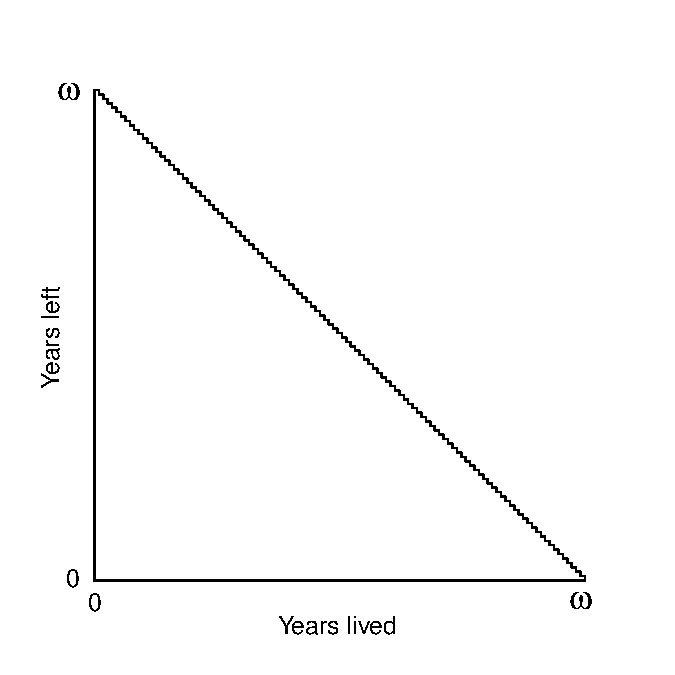
\includegraphics[scale=.7]{Figures/Triangle1}
\end{figure}
\end{frame}
\begin{frame}
\frametitle{Lifespans and time}
\vspace{-1cm}
\begin{figure}
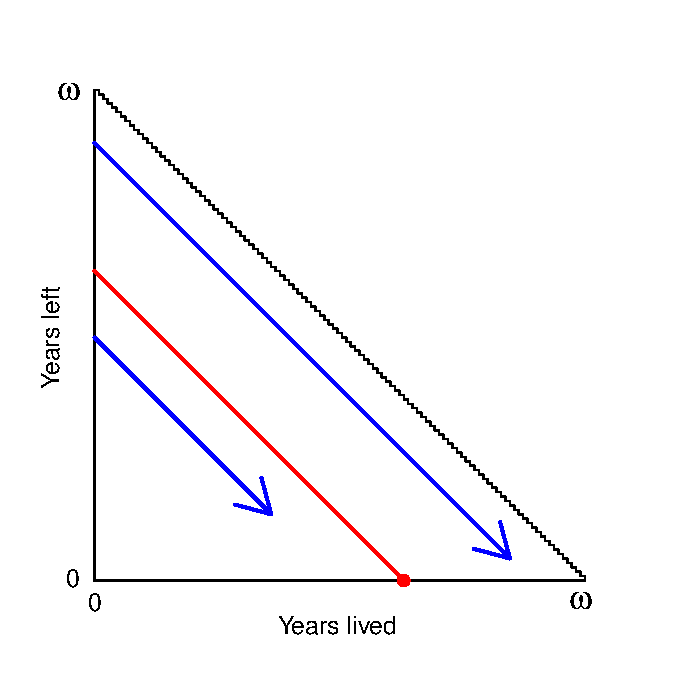
\includegraphics[scale=.7]{Figures/Triangle2}
\end{figure}
\end{frame}
\begin{frame}
\frametitle{Area examined}
\vspace{-1cm}
\begin{figure}
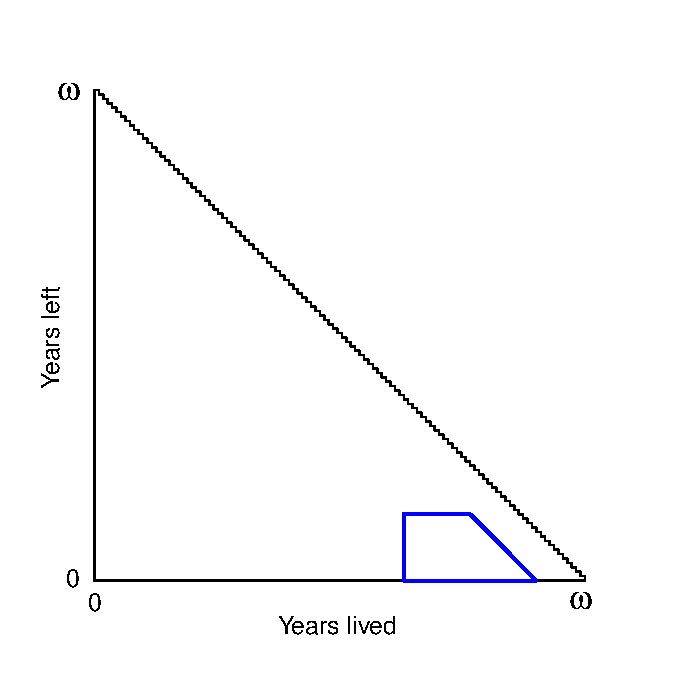
\includegraphics[scale=.7]{Figures/Triangle3}
\end{figure}
\end{frame}
%------------------------------------------------

\section{Data, descriptive method}

%------------------------------------------------

\begin{frame}
\frametitle{Data}
\begin{block}{US HRS}
10 waves spanning 20 years (1992-2011)\\
47530 observations of 11520 individuals observed until death, about 53\% female.
\end{block}
\end{frame}

%------------------------------------------------

\begin{frame}
\frametitle{Data, females}
\begin{figure}
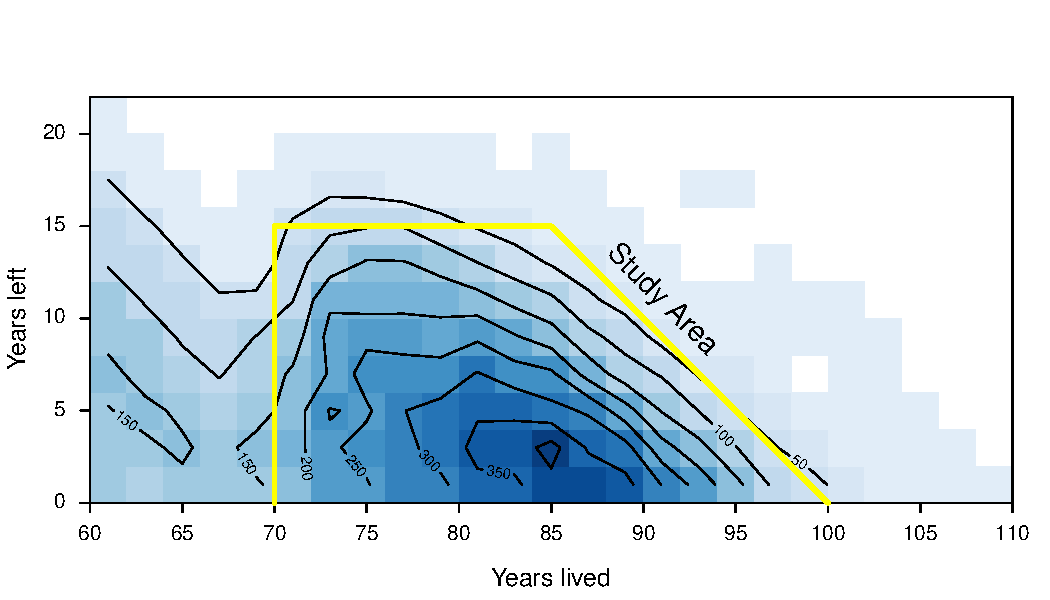
\includegraphics[width=\linewidth]{Figures/CaseCountFemales}
\end{figure}
\end{frame}

%------------------------------------------------

\begin{frame}
\frametitle{Data, males}
\begin{figure}
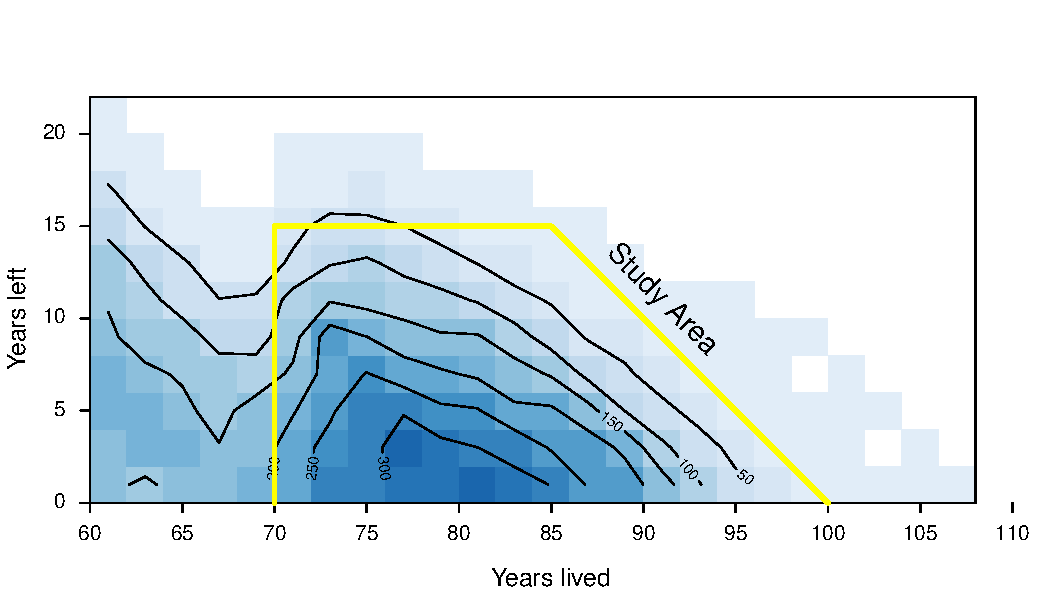
\includegraphics[width=\linewidth]{Figures/CaseCountMales}
\end{figure}
\end{frame}

%------------------------------------------------

\begin{frame}
\frametitle{Example: binned (ADL3, females)}
\begin{figure}
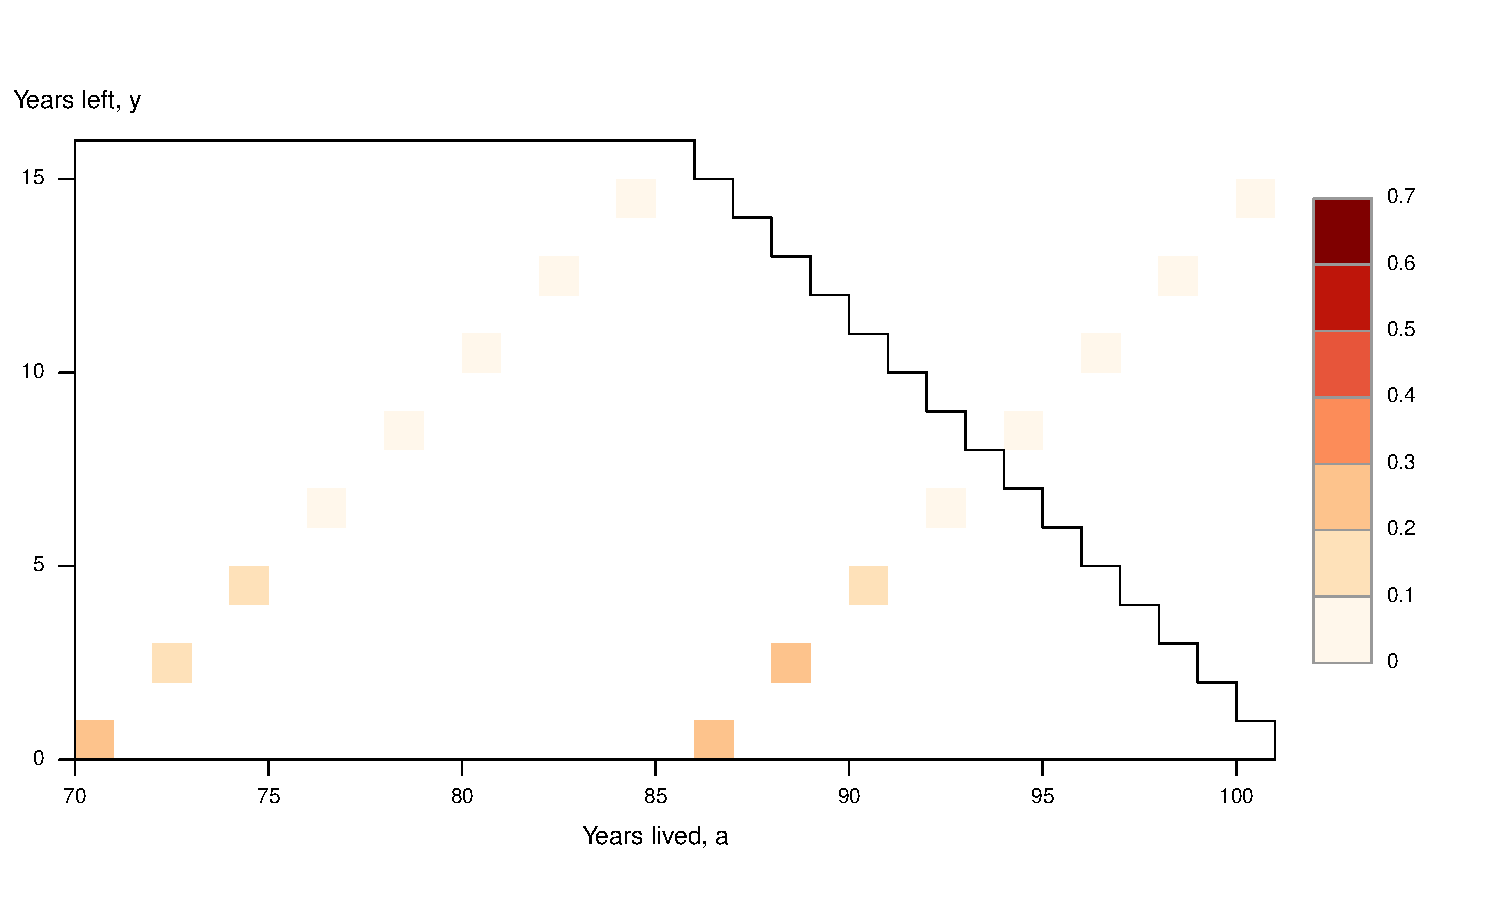
\includegraphics[width=\linewidth]{Figures/SurfExampleFemalesADL3_1}
\end{figure}
\end{frame}
\begin{frame}
\frametitle{Example: loess smoothed (ADL3, females)}
\begin{figure}
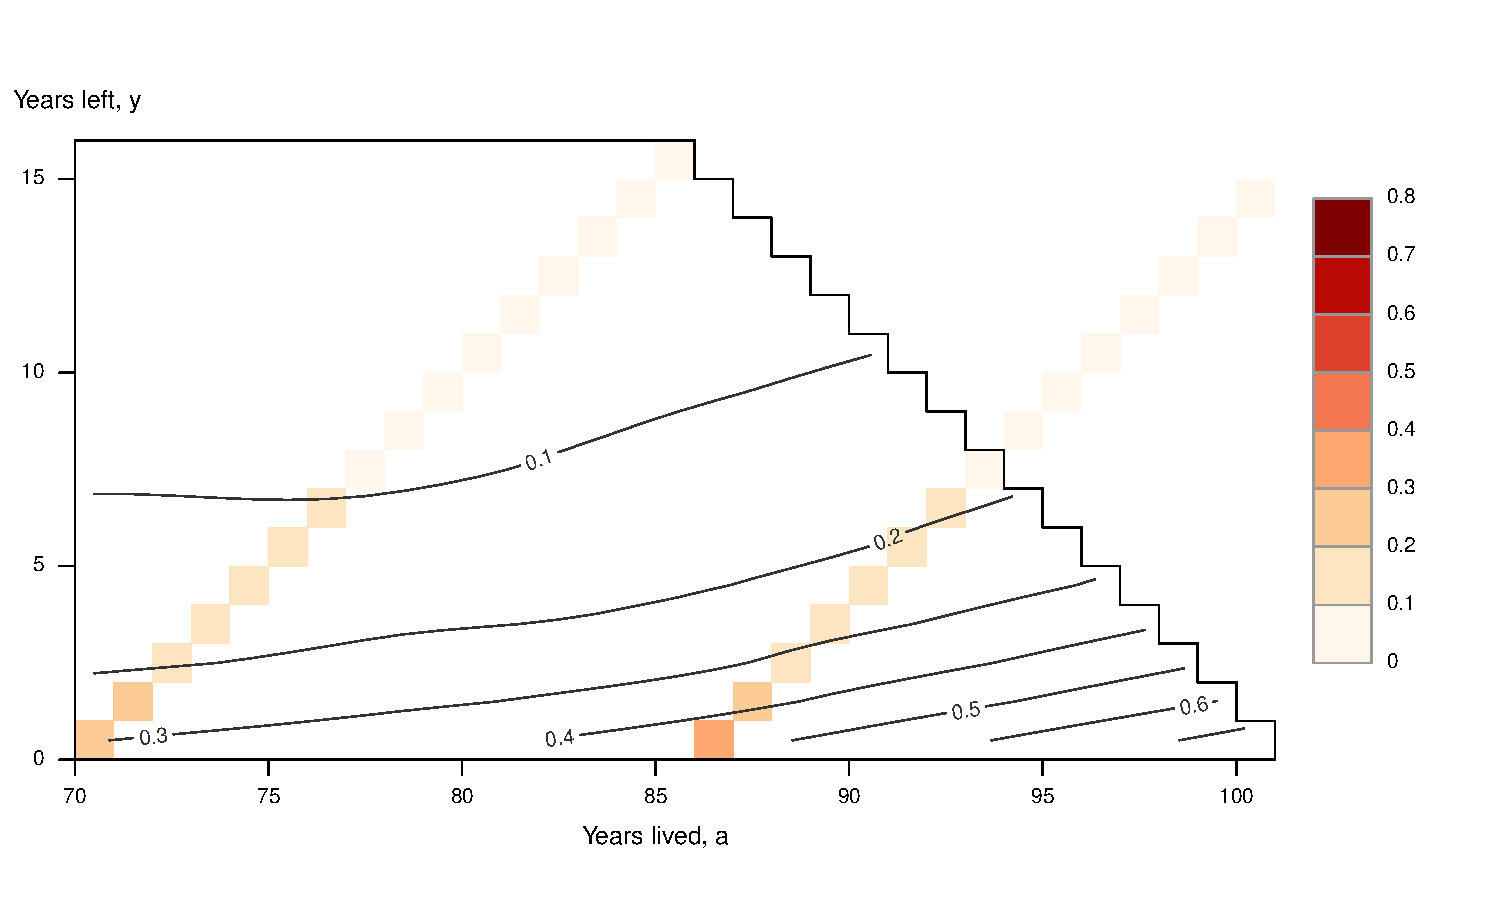
\includegraphics[width=\linewidth]{Figures/SurfExampleFemalesADL3_2}
\end{figure}
\end{frame}
\begin{frame}
\frametitle{Example: characterization (ADL3, females)}
\begin{figure}
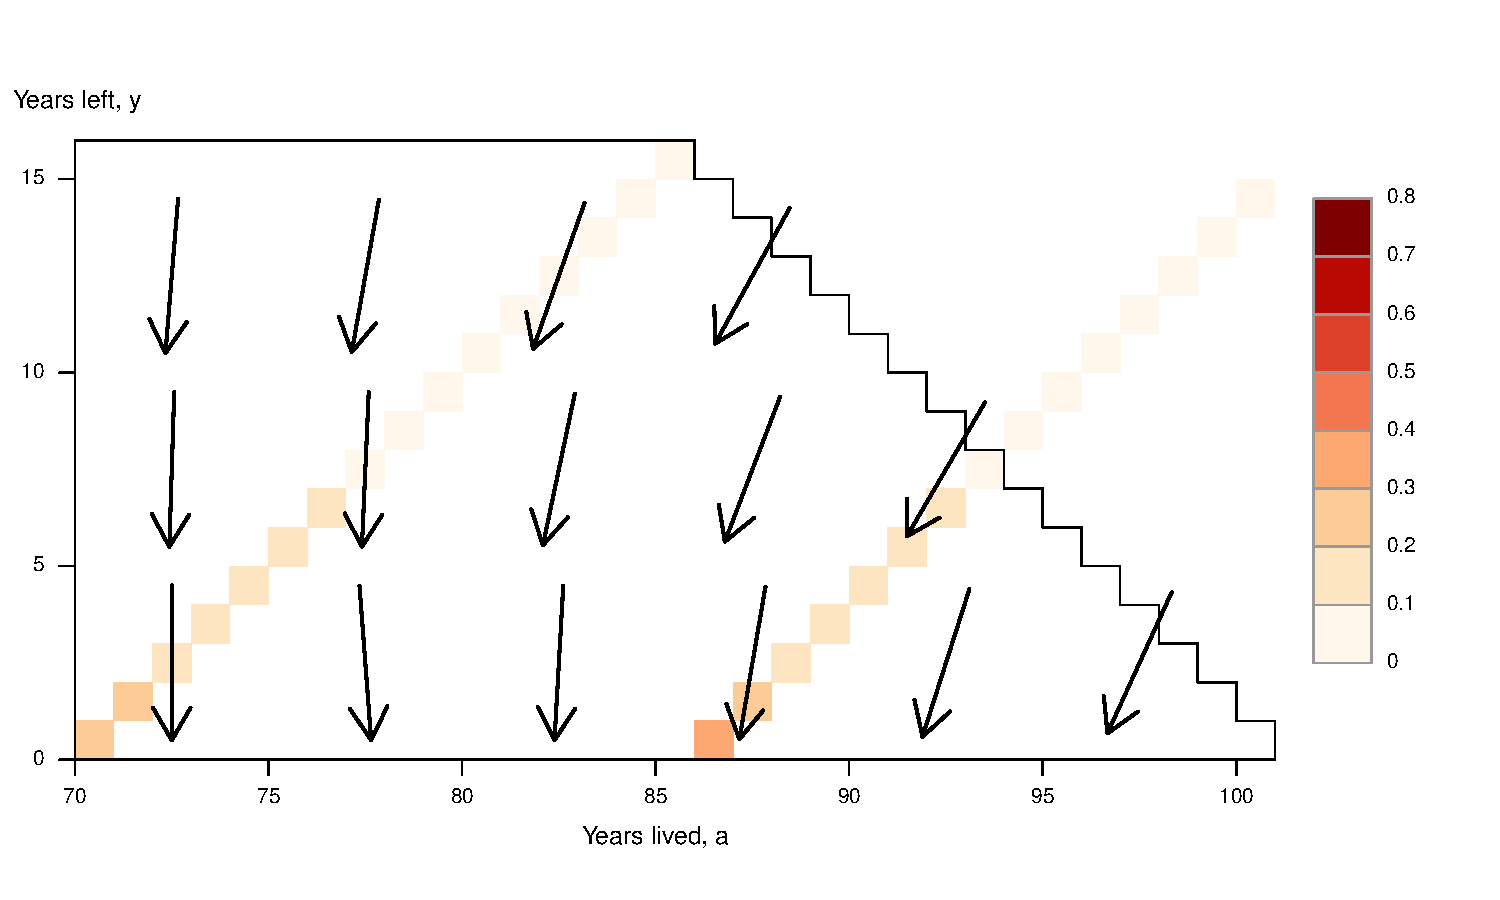
\includegraphics[width=\linewidth]{Figures/SurfExampleFemalesADL3_3}
\end{figure}
\end{frame}

\begin{frame}
\frametitle{Convert arrows to percent thanatological}
\vspace{-1em}
\begin{figure}
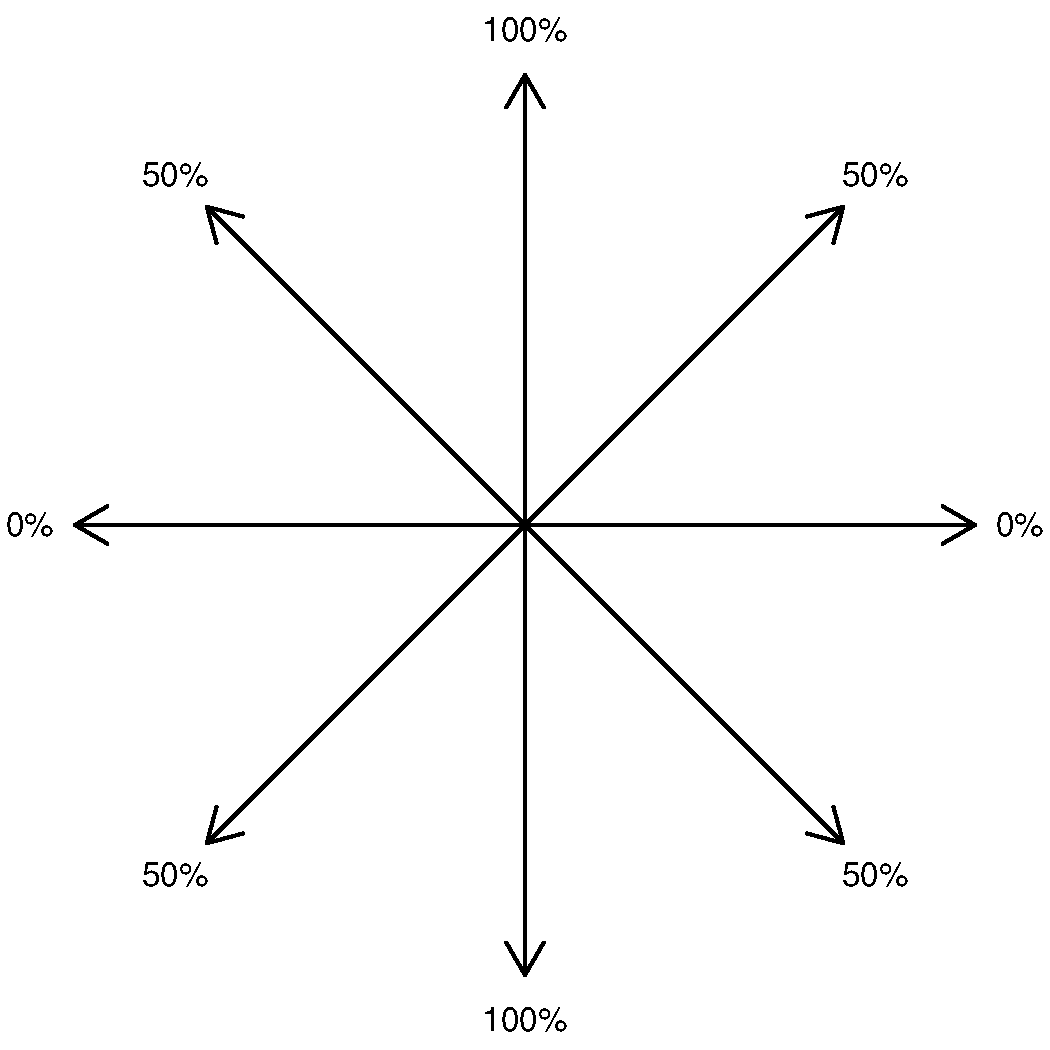
\includegraphics[width=.5\linewidth]{Figures/ArrowDiagram}
\end{figure}
\end{frame}

\begin{frame}
\frametitle{Example: summary (ADL3, females)}
\begin{itemize}
  	\item take mean percentage of all arrows
	\item for ADL3, females, we have 89\% vertical / 11\% horizontal.
	\item ADL3 is 89\% a TTD story (for this region of the age surface)
\end{itemize}
\end{frame}

% -----------------------------------------------
\begin{frame}
\frametitle{Characteristics explored}
\begin{itemize}
  \item ADL (8 items)
  \item IADL (9 items)
  \item Healthcare usage (9 items)
  \item Functional limitations (6 items)
  \item Health behaviors (5 items)
  \item Chronic conditions (9 items)
  \item Psychological conditions (10 items)
  \item Cognitive function (19 items)
\end{itemize}
\end{frame}

%------------------------------------------------

\section{Results}

%------------------------------------------------

\begin{frame}
\frametitle{Results summary}
\begin{figure}
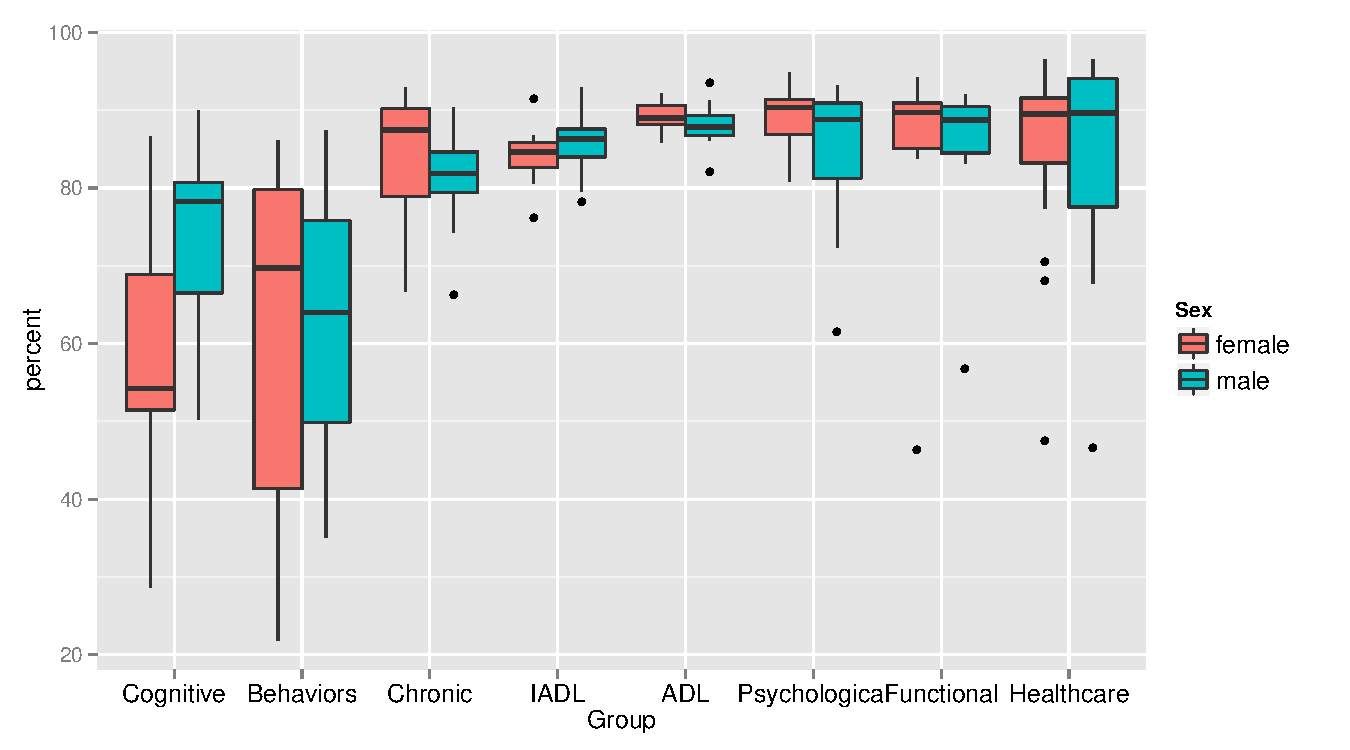
\includegraphics[width=.8\linewidth]{Figures/ResultsBoxplot}
\end{figure}
\end{frame}

%------------------------------------------------

\begin{frame}
\frametitle{Results (cont)}
\begin{itemize}
  \item All surfaces in one pdf file by email or USB
  \item tim.riffe@gmail.com
  \item Thanks!
\end{itemize}
\end{frame}

%----------------------------------------------------------------------------------------

\end{document}





